\documentclass[10pt,twocolumn]{article}
\usepackage[margin=0.8in]{geometry}
\usepackage{amsmath,amssymb,booktabs,graphicx,hyperref,xcolor,framed}
\hypersetup{colorlinks=true,linkcolor=blue!50!black,urlcolor=blue!50!black}
\setlength{\columnsep}{0.28in}
\newcommand{\ActA}{18}
\newcommand{\NptsA}{240}
\newcommand{\GaussA}{1.2\times10^{-8}}
\newcommand{\GaussHiA}{9.6\times10^{-8}}
\newcommand{\BianA}{7.6\times10^{-13}}
\newcommand{\BianHiA}{1.5\times10^{-10}}
\newcommand{\AsymA}{2.9\times10^{-10}}
\newcommand{\SplitA}{1.2\times10^{-15}}
\newcommand{\RconnVsGaussA}{4.8\times10^{-10}}
\newcommand{\EigMinA}{3.4\times10^{-4}}
\newcommand{\EigMaxA}{1.31}
\newcommand{\CondA}{4849}
\newcommand{\LegacyA}{1.74\times10^{3}}
\newcommand{\RmedA}{24.1}
\newcommand{\RloA}{-1027}
\newcommand{\RhiA}{6666}
\newcommand{\AbsRA}{307}
\newcommand{\KmedA}{3.8\times10^{-5}}
\newcommand{\KloA}{-0.007}
\newcommand{\KhiA}{0.022}
\newcommand{\KNegA}{45}
\newcommand{\GeoMsA}{0.60}
\newcommand{\GeoMeA}{1.90}
\newcommand{\GeoLenA}{6.263}
\newcommand{\LineLenA}{6.623}
\newcommand{\GeoNormalA}{94}
\newcommand{\LineNormalA}{3}
\newcommand{\GeoHawkA}{0.108}
\newcommand{\LineHawkA}{0.049}
\newcommand{\GeoEinA}{0.227}
\newcommand{\LineEinA}{0.101}
\newcommand{\GeoSpeedA}{2\times10^{-4}}
\newcommand{\RDustA}{-138.4}
\newcommand{\ShCoDustA}{$<$1}
\newcommand{\ShGrDustA}{14}
\newcommand{\ShQuDustA}{54}
\newcommand{\ShHoDustA}{19}
\newcommand{\ShPlDustA}{13}
\newcommand{\RRadiationA}{43.3}
\newcommand{\ShCoRadiationA}{$<$1}
\newcommand{\ShGrRadiationA}{12}
\newcommand{\ShQuRadiationA}{42}
\newcommand{\ShHoRadiationA}{28}
\newcommand{\ShPlRadiationA}{18}
\newcommand{\RVacuumA}{501.8}
\newcommand{\ShCoVacuumA}{$<$1}
\newcommand{\ShGrVacuumA}{13}
\newcommand{\ShQuVacuumA}{50}
\newcommand{\ShHoVacuumA}{18}
\newcommand{\ShPlVacuumA}{20}
\newcommand{\RBlackholeA}{-15.9}
\newcommand{\ShCoBlackholeA}{$<$1}
\newcommand{\ShGrBlackholeA}{27}
\newcommand{\ShQuBlackholeA}{21}
\newcommand{\ShHoBlackholeA}{32}
\newcommand{\ShPlBlackholeA}{19}
\newcommand{\RWormholeA}{363.4}
\newcommand{\ShCoWormholeA}{$<$1}
\newcommand{\ShGrWormholeA}{16}
\newcommand{\ShQuWormholeA}{37}
\newcommand{\ShHoWormholeA}{26}
\newcommand{\ShPlWormholeA}{21}
\newcommand{\RHawkingA}{-8.6}
\newcommand{\ShCoHawkingA}{$<$1}
\newcommand{\ShGrHawkingA}{25}
\newcommand{\ShQuHawkingA}{29}
\newcommand{\ShHoHawkingA}{28}
\newcommand{\ShPlHawkingA}{17}
\newcommand{\BerryA}{8\times10^{-16}}
\newcommand{\ActB}{18}
\newcommand{\NptsB}{240}
\newcommand{\GaussB}{1.6\times10^{-8}}
\newcommand{\GaussHiB}{1.7\times10^{-7}}
\newcommand{\BianB}{1.1\times10^{-12}}
\newcommand{\BianHiB}{8.2\times10^{-11}}
\newcommand{\AsymB}{4.2\times10^{-10}}
\newcommand{\SplitB}{1.2\times10^{-15}}
\newcommand{\RconnVsGaussB}{4.3\times10^{-10}}
\newcommand{\EigMinB}{2.2\times10^{-4}}
\newcommand{\EigMaxB}{1.29}
\newcommand{\CondB}{7562}
\newcommand{\LegacyB}{2.62\times10^{3}}
\newcommand{\RmedB}{-27.9}
\newcommand{\RloB}{-5496}
\newcommand{\RhiB}{3773}
\newcommand{\AbsRB}{524}
\newcommand{\KmedB}{7.8\times10^{-5}}
\newcommand{\KloB}{-0.006}
\newcommand{\KhiB}{0.025}
\newcommand{\KNegB}{41}
\newcommand{\GeoMsB}{0.60}
\newcommand{\GeoMeB}{1.90}
\newcommand{\GeoLenB}{6.205}
\newcommand{\LineLenB}{6.560}
\newcommand{\GeoNormalB}{97}
\newcommand{\LineNormalB}{5}
\newcommand{\GeoHawkB}{0.118}
\newcommand{\LineHawkB}{0.041}
\newcommand{\GeoEinB}{0.415}
\newcommand{\LineEinB}{0.084}
\newcommand{\GeoSpeedB}{6\times10^{-5}}
\newcommand{\RDustB}{-384.8}
\newcommand{\ShCoDustB}{$<$1}
\newcommand{\ShGrDustB}{14}
\newcommand{\ShQuDustB}{42}
\newcommand{\ShHoDustB}{26}
\newcommand{\ShPlDustB}{18}
\newcommand{\RRadiationB}{-143.4}
\newcommand{\ShCoRadiationB}{$<$1}
\newcommand{\ShGrRadiationB}{13}
\newcommand{\ShQuRadiationB}{38}
\newcommand{\ShHoRadiationB}{30}
\newcommand{\ShPlRadiationB}{18}
\newcommand{\RVacuumB}{-304.5}
\newcommand{\ShCoVacuumB}{$<$1}
\newcommand{\ShGrVacuumB}{8}
\newcommand{\ShQuVacuumB}{37}
\newcommand{\ShHoVacuumB}{31}
\newcommand{\ShPlVacuumB}{24}
\newcommand{\RBlackholeB}{-24.6}
\newcommand{\ShCoBlackholeB}{$<$1}
\newcommand{\ShGrBlackholeB}{22}
\newcommand{\ShQuBlackholeB}{21}
\newcommand{\ShHoBlackholeB}{34}
\newcommand{\ShPlBlackholeB}{22}
\newcommand{\RWormholeB}{519.8}
\newcommand{\ShCoWormholeB}{$<$1}
\newcommand{\ShGrWormholeB}{12}
\newcommand{\ShQuWormholeB}{35}
\newcommand{\ShHoWormholeB}{23}
\newcommand{\ShPlWormholeB}{29}
\newcommand{\RHawkingB}{-3.2}
\newcommand{\ShCoHawkingB}{$<$1}
\newcommand{\ShGrHawkingB}{28}
\newcommand{\ShQuHawkingB}{17}
\newcommand{\ShHoHawkingB}{34}
\newcommand{\ShPlHawkingB}{21}
\newcommand{\BerryB}{7\times10^{-16}}


\title{\vspace{-1.2em}\textbf{Field Equations of the Modak--Walawalkar Manifold, Version 2:\\
Einstein-Form Equations Read Off a Trained Manifold}\\[2pt]
\large Exploratory physics, November 2026}
\author{Rahul Modak$^{1}$ \quad Dr.\ Rahul Walawalkar$^{2}$\\[2pt]
\small $^1$Bayesian Cybersecurity Pvt.\ Ltd., Mumbai/Thane, India \quad
$^2$Carnegie Mellon University; NETRA; Caret Capital\\
\small Code: \url{https://github.com/RahulModak74/QUANTUM_GRAVITY_WITH_MW} (folder \texttt{Nov-2026\_tests/EXPLORATORY\_PHYSICS})\\
\small Supersedes \emph{Fundamental Field Equations of the Modak--Walawalkar Framework} (January 2026)}
\date{}

\begin{document}
\twocolumn[
\begin{@twocolumnfalse}
\maketitle
\begin{framed}
\small\textbf{Disclaimer.} We do not claim to have solved quantum gravity or any open problem in
physics. This note answers a narrower question: \emph{if the M-W manifold trained on joint GR+QM
data is taken as given, which differential equations does it satisfy, and can they be written
in the shape of Einstein's field equations?} Every equation below is a property of that learned
object, verified numerically on it. Whether it describes nature is a separate question that this
note does not address.
\end{framed}
\begin{abstract}
The usual order in physics is equations first, then numerics. Here the order is reversed: the
Nov-2026 M-W manifold (a 20-dimensional physics-prior VAE trained on six GR+QM regimes) is the
starting object, and its field equations are read off it with exact automatic derivatives. The
decoder is an immersion of the latent space into the standardised data space; its pullback
metric, Levi-Civita connection and second fundamental form are computed exactly, in float64,
at \NptsA{} unseen test states. The curvature satisfies an equation of exactly Einstein's form,
$G_{ab}=\kappa\,T^{\rm MW}_{ab}$, in which the source $T^{\rm MW}$ is built from the manifold's
extrinsic curvature and splits additively over gravity, quantum, horizon, coordinate and
Planck-flag columns. Two independent routes to the Riemann tensor agree to $\GaussA$ (median), the
contracted Bianchi identity $\nabla^aG_{ab}=0$ (hence $\nabla^aT^{\rm MW}_{ab}=0$) holds to
$\BianA$, and the column split is exact to $\SplitA$. A minimum-energy path between a light and a
heavy black hole satisfies the geodesic equation and passes through black holes of uniformly
increasing mass. We also correct three numerical errors in Version 1, whose headline
``$R=2.88\times10^{7}$'' was not a curvature.
\end{abstract}
\vspace{1em}
\end{@twocolumnfalse}
]

\section{The reverse workflow}
Standard practice writes partial differential equations (PDEs) first and then builds numerical
schemes to solve them. The M-W framework inverts this. The theories' constraints enter as Bayesian
priors, a VAE learns the joint density of valid states, and the resulting \emph{manifold} is the
object on which a new idea is tested. Only afterwards are the PDEs it obeys extracted, as here.
The idea goes from concept to tested object to equations in weeks rather than years, and the
object has 20 latent dimensions (\ActA{} of them active), well beyond the four or five
dimensions a person can construct by hand.

A PDE solver also works with geometry, but only locally: it evaluates tangents cell by cell and
the solver stitches the cells into a mesh. A learned manifold is the global object itself, a
smooth, differentiable chart at every point with exact derivatives on demand, so it acts as a
mesh of arbitrary resolution.

\section{The object}
Let $u\in U\subset\mathbb{R}^{n}$, $n=\ActA$, be the active latent axes of the Nov-2026 checkpoint
\texttt{A\_full\_prior} (the two axes with KL$<0.1$ carry no information and are held fixed). The
decoder $f:U\to\mathbb{R}^{30}$ maps a latent point to the 30 standardised data columns
(coordinates, metric and its fluctuations, $R$, $T_{\mu\nu}$, $\psi$, $M$, $r_s$, $T_H$, $S$,
uncertainty and Planck/topology flags). It is an immersion: $\partial_a f$ has full rank $n$ at
every test point (smallest metric eigenvalue median $\EigMinA$, condition number median $\CondA$).

\paragraph{Exact derivatives.} $f$, $\partial f$ and $\partial^2 f$ are propagated analytically
through every layer (Linear, LayerNorm, tanh), which is exact to round-off and agrees with
reverse-mode autodiff to $10^{-15}$. (Nested forward-mode autodiff through LayerNorm returned a
wrong Hessian in the PyTorch version used; this was detected by a finite-difference check.)

\section{Geometry of the manifold}
\begin{align}
g_{ab} &= \langle\partial_a f,\partial_b f\rangle, \label{eq:g}\\
\Gamma^{c}{}_{ab} &= g^{cd}\langle\partial_d f,\partial_a\partial_b f\rangle, \label{eq:gam}\\
\mathrm{II}_{ab} &= P_\perp\,\partial_a\partial_b f,\qquad P_\perp = I - (\partial f)\,g^{-1}(\partial f)^{\!\top},\label{eq:II}
\end{align}
with $\langle\cdot,\cdot\rangle$ the Euclidean product of $\mathbb{R}^{30}$ in standardised units.
The Riemann tensor follows from the Gauss equation,
\begin{equation}
R_{abcd}=\langle\mathrm{II}_{ac},\mathrm{II}_{bd}\rangle-\langle\mathrm{II}_{ad},\mathrm{II}_{bc}\rangle,
\label{eq:gauss}
\end{equation}
and independently from the connection,
$R^{a}{}_{bcd}=\partial_c\Gamma^a{}_{db}-\partial_d\Gamma^a{}_{cb}+\Gamma^a{}_{ce}\Gamma^e{}_{db}-\Gamma^a{}_{de}\Gamma^e{}_{cb}$,
with $\partial\Gamma$ taken by fourth-order central differences of the exact $\Gamma$.

\section{The field equation in Einstein's form}
Contracting (\ref{eq:gauss}) with $H\equiv g^{ab}\mathrm{II}_{ab}$ (mean-curvature vector) gives
\begin{equation}
\boxed{\;G_{ab}\equiv R_{ab}-\tfrac12 g_{ab}R=\kappa\,T^{\rm MW}_{ab}\;}
\label{eq:efe}
\end{equation}
\begin{equation}
\kappa T^{\rm MW}_{ab}=\langle H,\mathrm{II}_{ab}\rangle-g^{cd}\langle\mathrm{II}_{ac},\mathrm{II}_{bd}\rangle
-\tfrac12 g_{ab}\bigl(|H|^2-|\mathrm{II}|^2\bigr),
\label{eq:T}
\end{equation}
$\kappa=8\pi G$, $G=1$. Equation (\ref{eq:efe}) has exactly Einstein's shape: geometry on the left;
on the right a symmetric source built from how the manifold bends inside the data space.

\paragraph{Additive sources.} Because $\langle\cdot,\cdot\rangle$ is a sum over data columns, the
source splits exactly into column groups $s$:
\begin{equation}
G_{ab}=\kappa\sum_{s}T^{(s)}_{ab},\quad s\in\{\text{grav},\text{quant},\text{hor},\text{coord},\text{Planck}\}.
\label{eq:split}
\end{equation}
Gravity and quantum content enter one equation as additive terms. No coupling step is needed
between them.

\paragraph{Conservation.} The contracted Bianchi identity $\nabla^aG_{ab}=0$ implies
\begin{equation}
\nabla^aT^{\rm MW}_{ab}=0,
\label{eq:cons}
\end{equation}
the analogue of $\nabla^\mu T_{\mu\nu}=0$ in GR.

\paragraph{Geodesic equation.} Free motion on the manifold obeys
\begin{equation}
\ddot u^{c}+\Gamma^{c}{}_{ab}\dot u^{a}\dot u^{b}=0
\;\Longleftrightarrow\; P_{\parallel}\,\ddot{x}=0,\quad x=f(u),
\label{eq:geo}
\end{equation}
i.e.\ a geodesic's data-space acceleration is purely normal to the manifold.

\section{Verification on the trained manifold}
\begin{table}[h]\centering\small
\begin{tabular}{@{}lcc@{}}\toprule
Check (median over test states) & with priors & no priors\\\midrule
Gauss: Riem$(\Gamma)$ vs Riem(II) & $\GaussA$ & $\GaussB$\\
Bianchi $|\nabla^aG_{ab}|$ / scale & $\BianA$ & $\BianB$\\
Ricci asymmetry (from $\Gamma$) & $\AsymA$ & $\AsymB$\\
Source split (\ref{eq:split}) & $\SplitA$ & $\SplitB$\\\bottomrule
\end{tabular}
\caption{Residuals of the identities (\ref{eq:gauss})--(\ref{eq:cons}) at $\NptsA$ unseen test
states (40 per regime). 95th percentiles: Gauss $\GaussHiA$, Bianchi $\BianHiA$.}
\label{tab:checks}
\end{table}

\paragraph{Numerical values.} Ricci scalar median $\RmedA$ (5--95\%: $\RloA$ to $\RhiA$; median
$|R|=\AbsRA$). Sectional curvatures of coordinate planes are small and of both signs (median
$\KmedA$, 5--95\% $[\KloA,\KhiA]$, $\KNegA\%$ negative): the manifold is nearly flat along most
planes and curved along a few. Median $R$ by regime: dust $\RDustA$, radiation $\RRadiationA$,
vacuum $\RVacuumA$, black hole $\RBlackholeA$, wormhole $\RWormholeA$, Hawking $\RHawkingA$.
Figure~\ref{fig:main}(b,c) shows the spread and the source shares.

\paragraph{Geodesic between black holes.} We minimised the discrete path energy between a black
hole with $M=\GeoMsA$ and one with $M=\GeoMeA$ (both inside the training range). The path is
shorter than the straight latent line ($\GeoLenA$ vs $\LineLenA$ in data units), has constant speed,
and $\GeoNormalA\%$ of its acceleration is normal to the manifold, compared with $\LineNormalA\%$ for
the straight line, which is the geodesic signature (\ref{eq:geo}). The decoded mass increases
uniformly along the geodesic (Fig.~\ref{fig:main}d): the geodesic between two black holes is a
continuous family of black holes. The Hawking relation holds along it to
$|8\pi M T_H-1|=\GeoHawkA$ (straight latent line: $\LineHawkA$).

\begin{figure*}[t]\centering
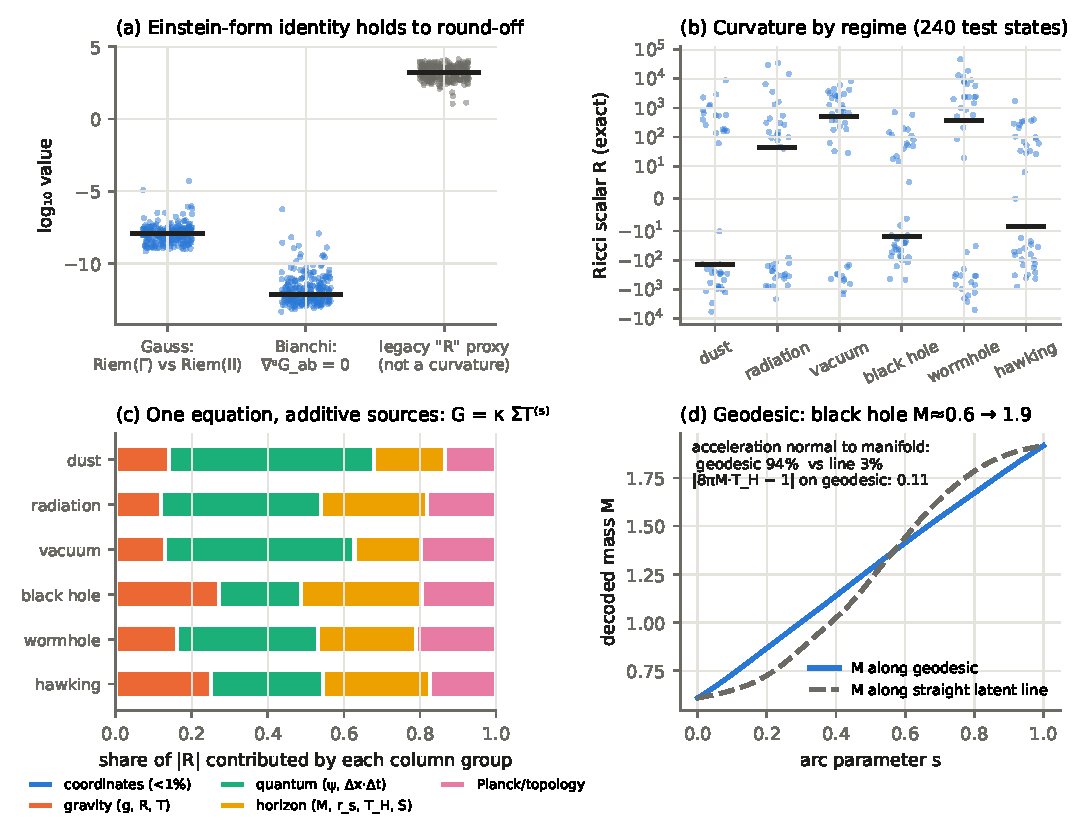
\includegraphics[width=0.86\textwidth]{fig_exploratory.pdf}
\caption{(a) Residuals of the Gauss and Bianchi identities versus the Version-1 curvature proxy.
(b) Exact Ricci scalar at 240 unseen test states. (c) Share of $|R|$ contributed by each column
group, Eq.~(\ref{eq:split}). (d) Decoded mass along the geodesic between a light and a heavy black
hole, and along the straight latent line. Checkpoint \texttt{A\_full\_prior}.}
\label{fig:main}
\end{figure*}

\section{Corrections to Version 1}
Re-running the January 2026 extraction scripts unchanged on the new manifold located three
errors.
\begin{enumerate}\itemsep0pt
\item The reported ``Ricci scalar'' $R=(2.88\pm1.80)\times10^{7}$ was the proxy
$\tfrac12(\log\det g+\operatorname{tr}g^{-1}-n)$, not a curvature. It is dominated by the inverse
of the smallest metric eigenvalue, which comes from latent axes the VAE does not use. On the new
manifold this proxy gives $\LegacyA$; the exact $|R|$ median is $\AbsRA$.
\item Christoffel symbols were formed from differences between consecutive \emph{random} latent
samples, which are not neighbouring points, so they carry no geometric meaning.
\item The Ricci formula kept only $\Gamma\Gamma-\Gamma\Gamma$ terms that are antisymmetric in
$(i,j)$; its trace with $g^{ij}$ is identically zero (the rerun returns $-1.3\times10^{-13}$).
\end{enumerate}
The Version-1 ``3.3\% Einstein residual'' came from the March 2026 (v4) pipeline. The
corrected v5 value is 1.3\%, reported in the Nov-2026 paper. The Version-1 equations for a quantum
connection $A_i$, the Euler-characteristic constraint and the unified tensor $\mathcal{R}_{IJ}$
were not extracted from the manifold and are not carried forward here. The companion note
\emph{Quantum Mechanics as Geometry, Version 2} computes the connection built from the decoded
wavefunction and finds it pure gauge.

\section{Scope}
Equation (\ref{eq:efe}) is an identity of any smooth immersed manifold. What the trained manifold
supplies is \emph{which} manifold: its metric, its curvature and the composition of its source
come from GR+QM data and the M-W priors. The latent coordinates are not spacetime coordinates, the
ambient metric is the Euclidean metric of standardised data, and the training data are synthetic.
The note shows that a learned manifold can be converted mechanically into field equations of
Einstein's form, with every term computable and checked. That is the claim, and the only claim.

\section*{Reproduce}
\small\texttt{cd Nov-2026\_tests/EXPLORATORY\_PHYSICS/code \&\& python3 mw\_exact\_geometry.py \&\&
python3 mw\_berry\_check.py \&\& python3 mw\_exact\_figures.py \&\& python3 mw\_paper\_numbers.py}
(about 15 min on a laptop CPU). Code implementation was assisted by AI coding tools; modelling
choices and claims are the authors'.
\end{document}
